\documentclass[utf8x]{beamer}

% This file is a solution template for:

% - Talk at a conference/colloquium.
% - Talk length is about 20min.
% - Style is ornate.

\mode<presentation>
{
  \usetheme{Warsaw}
  % or ...

  %\setbeamercovered{transparent}
  % or whatever (possibly just delete it)
}


\usepackage[english]{babel}
\usepackage{fancyvrb}
\usepackage{listings}
\usepackage{ulem}
\usepackage{color}
\usepackage{alltt}


\usepackage[T1]{fontenc}
\usepackage{setspace}
\usepackage[scaled=0.81]{beramono}
\definecolor{gray}{rgb}{0.3,0.3,0.3}

\lstset{
  basicstyle=\setstretch{1.05}\ttfamily\footnotesize,
  language=Python,
  keywordstyle=\bfseries,
  stringstyle=\color{blue},
  commentstyle=\color{gray}\textit,
  fancyvrb=true,
  showstringspaces=false,
  %keywords={def,while,if,elif,return,class,get,set,new,guard_class}
  numberstyle = \tiny,
  numbersep = -20pt,
}


\usepackage[utf8x]{inputenc}


\newcommand\redsout[1]{{\color{red}\sout{\hbox{\color{black}{#1}}}}}

% or whatever

% Or whatever. Note that the encoding and the font should match. If T1
% does not look nice, try deleting the line with the fontenc.


\title{Loop-Aware Optimizations in PyPy’s Tracing JIT}

\author[Ardö, Bolz, Fijałkowski]{\emph{Håkan Ardö}$^1$ \and \emph{Carl Friedrich Bolz}$^2$ \and Maciej Fijałkowski}
% - Give the names in the same order as the appear in the paper.
% - Use the \inst{?} command only if the authors have different
%   affiliation.

\institute[Lund, Düsseldorf]{
$^1$Centre for Mathematical Sciences, Lund University \and
$^2$Heinrich-Heine-Universität Düsseldorf, STUPS Group, Germany
}

\date{2012 DLS, 22nd of October, 2012}
% - Either use conference name or its abbreviation.
% - Not really informative to the audience, more for people (including
%   yourself) who are reading the slides online


% If you have a file called "university-logo-filename.xxx", where xxx
% is a graphic format that can be processed by latex or pdflatex,
% resp., then you can add a logo as follows:




% Delete this, if you do not want the table of contents to pop up at
% the beginning of each subsection:
%\AtBeginSubsection[]
%{
%  \begin{frame}<beamer>
%    \frametitle{Outline}
%    \tableofcontents[currentsection,currentsubsection]
%  \end{frame}
%}


% If you wish to uncover everything in a step-wise fashion, uncomment
% the following command: 

%\beamerdefaultoverlayspecification{<+->}


\begin{document}

\begin{frame}
  \titlepage
\end{frame}

\begin{frame}
  \frametitle{RPython and PyPy}
  \begin{itemize}
      \item Context: RPython
      \item a language for writing interpreters for dynamic languages
      \item a generic tracing JIT, applicable to many languages
      \item used to implement PyPy, an efficient Python interpreter
  \end{itemize}
\end{frame}

\begin{frame}
  \frametitle{Tracing JITs Compile by Observing an Interpreter}
  \begin{itemize}
      \item VM contains both an interpreter and the tracing JIT compiler
      \item JIT works by observing and logging what the interpreter does
      \item for interesting, commonly executed code paths
      \item produces a linear list of operations (trace)
  \end{itemize}
\end{frame}

\begin{frame}
  \frametitle{Why do tracing JITs work?}
  \begin{itemize}
      \item They are good at selecting interesting and common code paths
      \item both through the user program and through the runtime
      \item the latter is particularly important for dynamic languages with a big runtime like Python
          \pause
      \item traces are trivial to optimize
  \end{itemize}
\end{frame}

\begin{frame}
  \frametitle{Optimizing traces}
  \begin{itemize}
      \item A trace is an extended basic block
      \item (it has one entry and several exits)
      \item traces are easy to optime due to lack of control flow merges
          \pause
      \item most optimizations are one forward pass
      \item optimizers are often like symbolic executors
      \item can do optimizations that are expensive or even untractable with full control flow
  \end{itemize}
\end{frame}

\begin{frame}
  \frametitle{Example}
  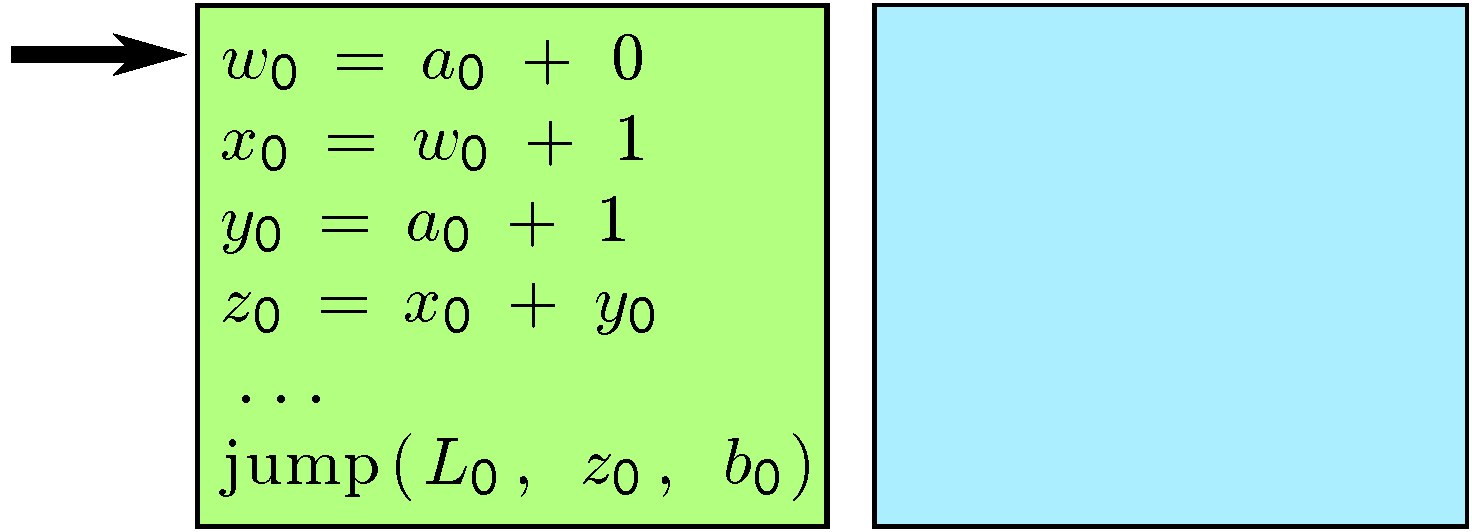
\includegraphics[width=\columnwidth]{figures/optimization1}
\end{frame}

\begin{frame}
  \frametitle{Example}
  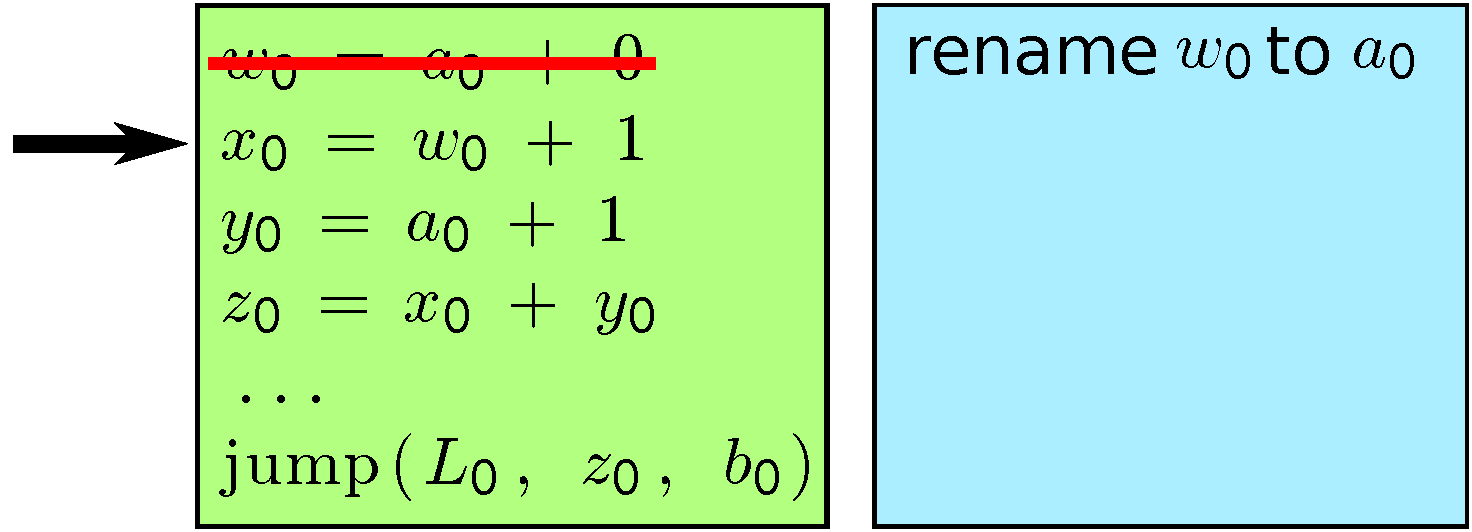
\includegraphics[width=\columnwidth]{figures/optimization2}
\end{frame}

\begin{frame}
  \frametitle{Example}
  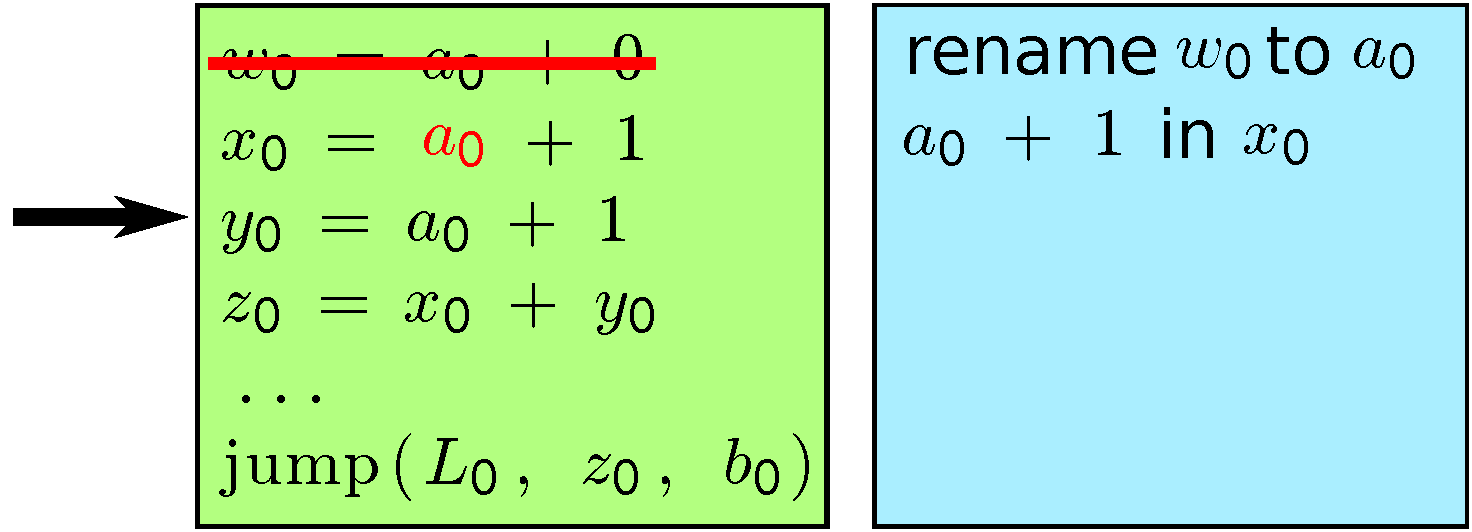
\includegraphics[width=\columnwidth]{figures/optimization3}
\end{frame}

\begin{frame}
  \frametitle{Example}
  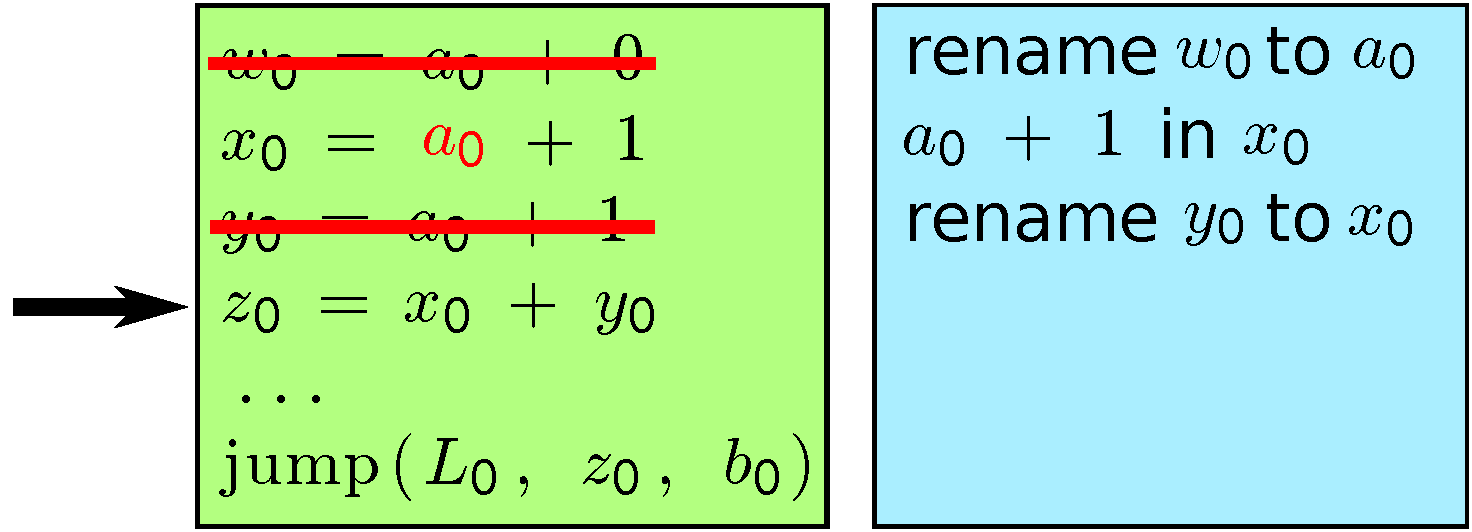
\includegraphics[width=\columnwidth]{figures/optimization4}
\end{frame}

\begin{frame}
  \frametitle{Example}
  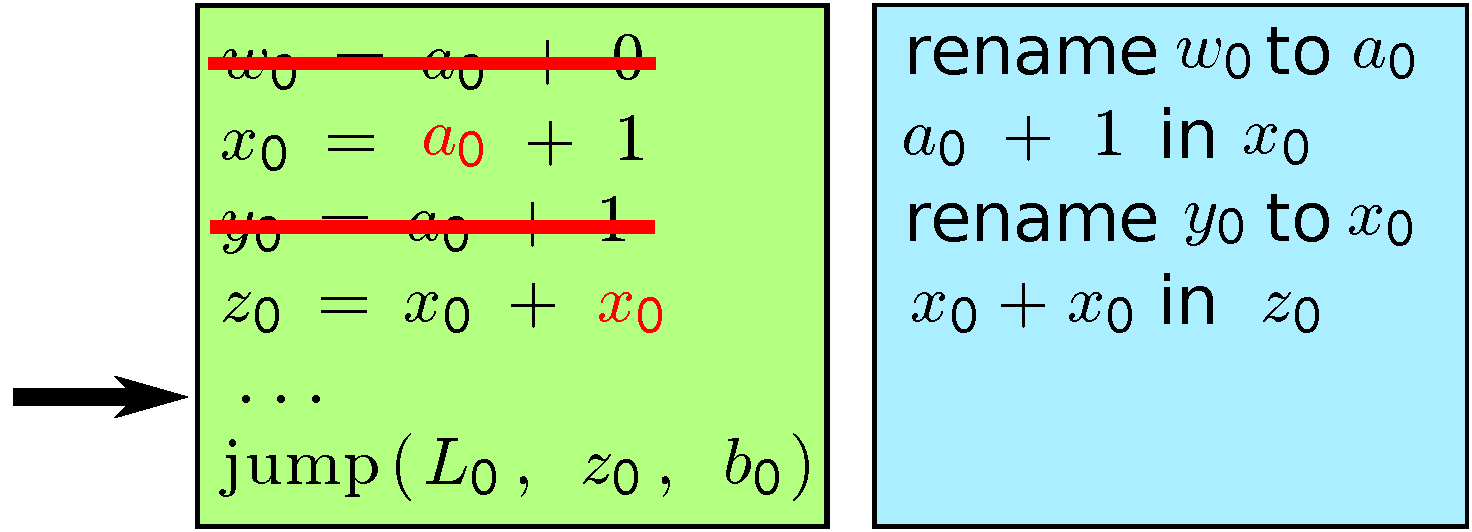
\includegraphics[width=\columnwidth]{figures/optimization5}
\end{frame}


\begin{frame}
  \frametitle{Problems with this approach}
  \begin{itemize}
      \item most traces actually are loops
      \item naive foward passes ignore this bit of control flow optimization available
      \item how to fix that without sacrifing simplicity of optimizations?
  \end{itemize}
\end{frame}

\begin{frame}
  \frametitle{Idea for solution}
  \begin{itemize}
      \item idea first proposed and implemented in LuaJIT by Mike Pall
      \item this talk presents the implementation of the same approach in RPython's tracing JIT
  \end{itemize}
  \pause
  \begin{block}{Approach}
      \begin{itemize}
          \item do a pre-processing step on the traces
          \item apply the unchanged forward-pass optimizations
          \item do some post-processing
          \item pre-processing is done in such a way that the normal optimizations become loop-aware
          \pause
          \item intuition: give the optimizations a second iteration of context to work with
      \end{itemize}
  \end{block}
\end{frame}

\begin{frame}
  \frametitle{Pre-processing the loops}
  \begin{itemize}
      \item pre-processing does loop unrolling
      \item peels off one iteration of the loop, duplicating the trace
      \item the optimizations optimize both iterations together
      \item this yields loop-invariant code motion and related optimizations
  \end{itemize}
\end{frame}

\begin{frame}
  \frametitle{Loop Peeling}
\begin{center}
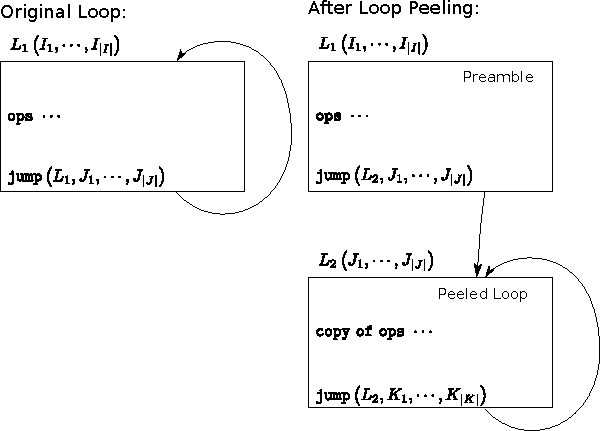
\includegraphics[width=\columnwidth]{../figures/overview}
\end{center}
\end{frame}


\begin{frame}[fragile]
  \frametitle{Loop Peeling}
    \begin{columns}
    \begin{column}{0.5\textwidth}
      \centering
            \begin{lstlisting}[mathescape]%,numbers = right,basicstyle=\setstretch{1.05}\ttfamily\scriptsize]
            abc
            $L_0$($i_{0}$):
            $i_1$ = $i_0$ + 1
            print($i_1$)
            jump($L_0$, $i_0$)
            $$
            $$
            $$
            $$
            $$
            \end{lstlisting}
    \end{column}
    \pause
    \begin{column}{0.5\textwidth}
      \centering
            \begin{lstlisting}[mathescape]%,numbers = right,basicstyle=\setstretch{1.05}\ttfamily\scriptsize]
            abc
            $L_0$($i_{0}$):
            $i_1$ = $i_0$ + 1
            print($i_1$)
            jump($L_1$, $i_0$)

            $L_1$($i_{0}$):
            $i_2$ = $i_0$ + 1
            print($i_2$)
            jump($L_1$, $i_0$)
            \end{lstlisting}
    \end{column}
  \end{columns}
\end{frame}

\begin{frame}[fragile]
  \frametitle{Apply Optimizations}
    \begin{columns}
    \begin{column}{0.5\textwidth}
      \centering
            \begin{lstlisting}[mathescape]%,numbers = right,basicstyle=\setstretch{1.05}\ttfamily\scriptsize]
            abc
            $L_0$($i_{0}$):
            $i_1$ = $i_0$ + 1
            print($i_1$)
            jump($L_1$, $i_0$)

            $L_1$($i_{0}$):
            $i_2$ = $i_0$ + 1
            print($i_2$)
            jump($L_1$, $i_0$)
            \end{lstlisting}
    \end{column}
    \pause
    \begin{column}{0.5\textwidth}
      \centering
            \begin{lstlisting}[mathescape]%,numbers = right,basicstyle=\setstretch{1.05}\ttfamily\scriptsize]
            abc
            $L_0$($i_{0}$):
            $i_1$ = $i_0$ + 1
            print($i_1$)
            jump($L_1$, $i_0$)

            $L_1$($i_{0}$):
            print($i_1$)
            jump($L_1$, $i_0$)
            \end{lstlisting}
    \end{column}
  \end{columns}
\end{frame}

\begin{frame}[fragile]
  \frametitle{Add extra arguments}
    \begin{columns}
    \begin{column}{0.5\textwidth}
      \centering
            \begin{lstlisting}[mathescape]%,numbers = right,basicstyle=\setstretch{1.05}\ttfamily\scriptsize]
            abc
            $L_0$($i_{0}$):
            $i_1$ = $i_0$ + 1
            print($i_1$)
            jump($L_1$, $i_0$)

            $L_1$($i_{0}$):
            print($i_1$)
            jump($L_1$, $i_0$)
            \end{lstlisting}
    \end{column}
    \pause
    \begin{column}{0.5\textwidth}
      \centering
            \begin{lstlisting}[mathescape]%,numbers = right,basicstyle=\setstretch{1.05}\ttfamily\scriptsize]
            abc
            $L_0$($i_{0}$):
            $i_1$ = $i_0$ + 1
            print($i_1$)
            jump($L_1$, $i_0$, $i_1$)

            $L_1$($i_{0}$, $i_1$):
            print($i_1$)
            jump($L_1$, $i_0$, $i_1$)
            \end{lstlisting}
    \end{column}
  \end{columns}
\end{frame}

\begin{frame}
  \frametitle{Optimizations helped by loop peeling}
  \begin{itemize}
      \item redundant guard removal
      \item common subexpression elimination
      \item heap optimizations
      \item allocation removal
  \end{itemize}
\end{frame}


\begin{frame}[fragile]
  \frametitle{Larger example}
    \begin{columns}
    \begin{column}{0.5\textwidth}
  \begin{lstlisting}
   while True:
      y = y + 1
  \end{lstlisting}
  \end{column}
    \pause
    \begin{column}{0.5\textwidth}
\begin{lstlisting}[mathescape]
$L_0$($p_{0}$, $p_{1}$):
guard_class($p_{1}$, BoxedInteger)
$i_{2}$ = get($p_{1}$, intval)
guard_class($p_{0}$, BoxedInteger)
$i_{3}$ = get($p_{0}$, intval)
$i_{4}$ = $i_{2} + i_{3}$
$p_{5}$ = new(BoxedInteger)
set($p_{5}$, intval, $i_{4}$)
jump($L_0$, $p_{0}$, $p_{5}$)
\end{lstlisting}
  \end{column}
  \end{columns}
\end{frame}


\begin{frame}[fragile]
  \frametitle{Peeled trace}
\begin{lstlisting}[mathescape]
$L_0$($p_{0}$, $p_{1}$):
guard_class($p_{1}$, BoxedInteger)
$i_{2}$ = get($p_{1}$, intval)
guard_class($p_{0}$, BoxedInteger)
$i_{3}$ = get($p_{0}$, intval)
$i_{4}$ = $i_{2}+i_{3}$
$p_{5}$ = new(BoxedInteger)
set($p_{5}$, intval, $i_{4}$)
jump($L_1$, $p_{0}$, $p_{5}$)

$L_1$($p_{0}$, $p_{5}$):
guard_class($p_{5}$, BoxedInteger)
$i_{6}$ = get($p_{5}$, intval)
guard_class($p_{0}$, BoxedInteger)
$i_{7}$ = get($p_{0}$, intval)
$i_{8}$ = $i_{6}+i_{7}$
$p_{9}$ = new(BoxedInteger)
set($p_{9}$, intval, $i_{8}$)
jump($L_1$, $p_{0}$, $p_{9}$)
\end{lstlisting}
\end{frame}

\begin{frame}[fragile]
  \frametitle{Final trace}
\begin{lstlisting}[mathescape]
$L_0$($p_{0}$, $p_{1}$):
guard_class($p_{1}$, BoxedInteger)
$i_{2}$ = get($p_{1}$, intval)
guard_class($p_{0}$, BoxedInteger)
$i_{3}$ = get($p_{0}$, intval)
$i_{4}$ = $i_{2}+i_{3}$
jump($L_1$, $p_{0}$, $i_{4}$)

$L_1$($p_{0}$, $i_{3}$, $i_{4}$):
$i_{8}$ = $i_{4}+i_{3}$
jump($L_1$, $p_{0}$, $i_{3}$, $i_8$)
\end{lstlisting}
\end{frame}



\begin{frame}
  \frametitle{Results}
  \begin{itemize}
      \item a number of numeric kernels
      \item some for image processing
      \item some from SciMark
      \item comparison against GCC and LuaJIT
      \pause
      \item geometric mean of speedups of loop peeling is 70\%
  \end{itemize}
\end{frame}

\begin{frame}
  \frametitle{Benchmark Results}
  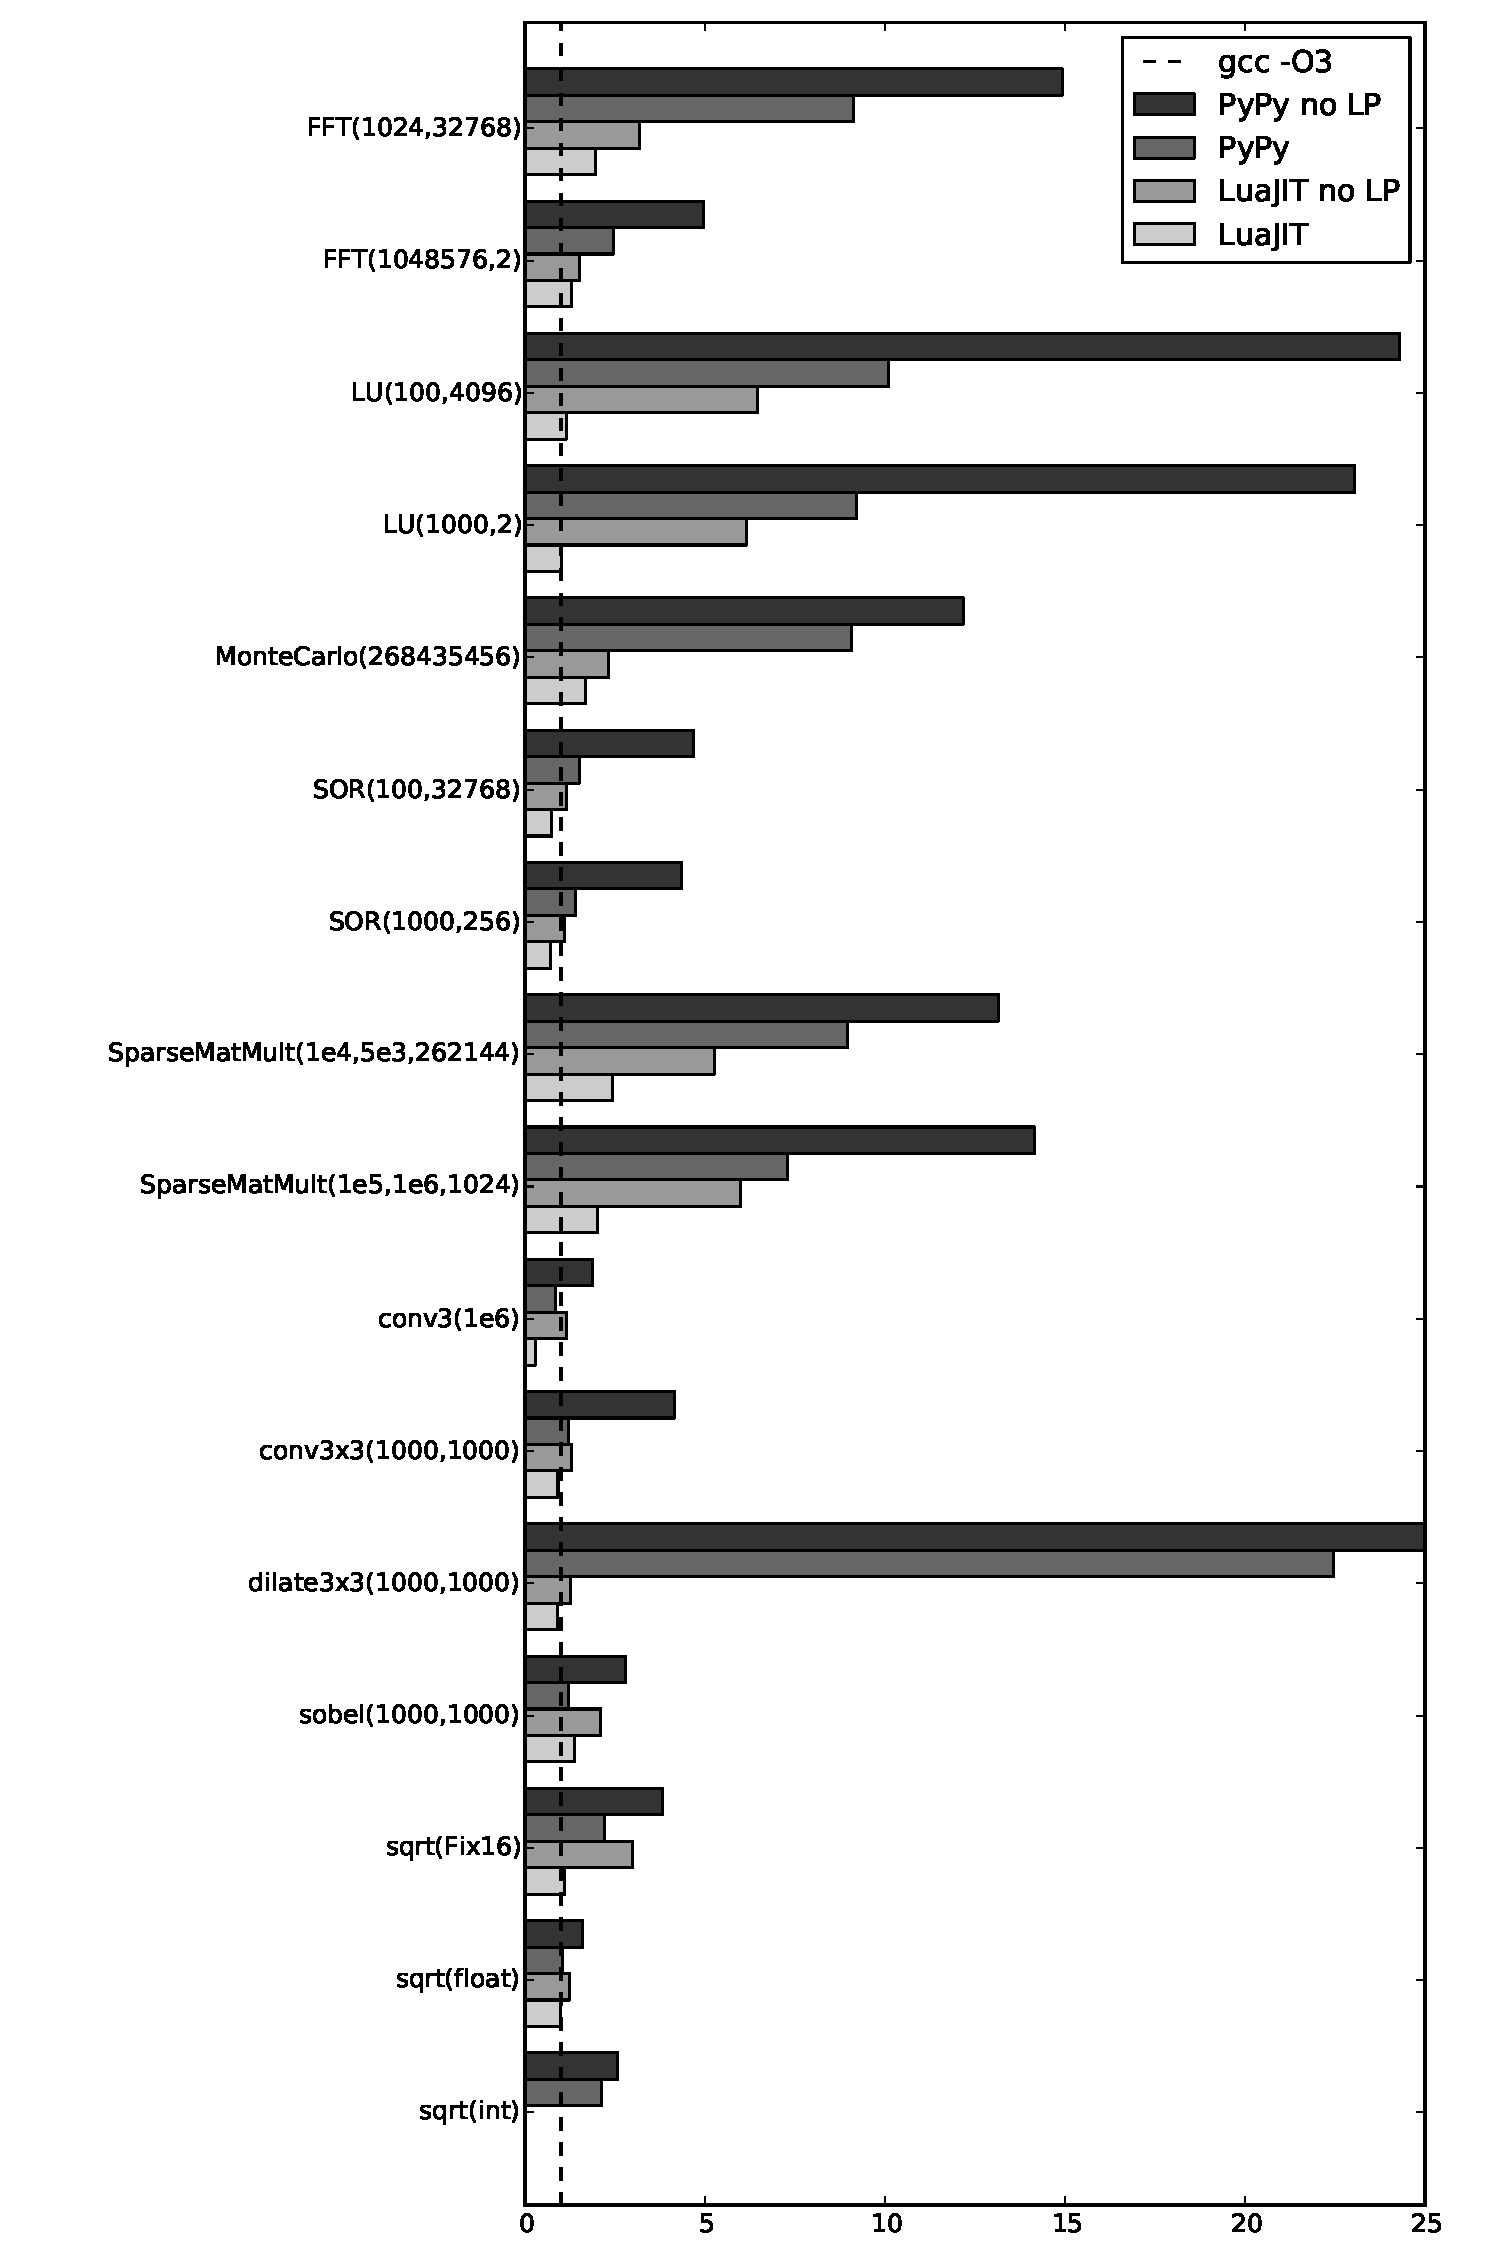
\includegraphics[width=0.7\textwidth,angle=90]{../benchmarks/result}
\end{frame}

\begin{frame}
  \frametitle{Conclusion}
  \begin{itemize}
      \item a simple preprocessing step on traces enables loop-aware optimizations for tracing JITs
      \item only minimal changes to the existing optimizations necessary
  \end{itemize}
\end{frame}



\begin{frame}
  \frametitle{Demo}
  \vfill
  \begin{itemize}
      \item Video analytics research example
      \item Experimenten driven - prototyping
      \item Custom loops over the pixels
      \item Good enough performace
  \end{itemize}
  \vfill
  \begin{itemize}
      \item Image class with task specific features
        \begin{itemize}
            \item Zero-padded
            \item Clips updates outside border
        \end{itemize}
      \item @autoreload decorator reloading functions on code change
      \item ReloadHack class reloads and reinstanciates on code change
  \end{itemize}
  \vfill
\end{frame}

\begin{frame}[fragile]
  \frametitle{Image class}
\begin{lstlisting}[mathescape,basicstyle=\setstretch{1.05}\ttfamily\scriptsize]
class Image(object):
    def __getitem__(self, (x, y)):
        if 0 <= x < self.width and 0 <= y < self.height:
            return self.data[y * self.width + x]
        return 0

    def __setitem__(self, (x, y), value):
        if 0 <= x < self.width and 0 <= y < self.height:
            self.data[y * self.width + x] = value

    __add__ = binop(float.__add__)
    __sub__ = binop(float.__sub__)
    __mul__ = binop(float.__mul__)
    __div__ = binop(float.__div__)
    __pow__ = binop(float.__pow__)

   ...
\end{lstlisting}
\end{frame}

\begin{frame}[fragile]
  \frametitle{Image class}
\begin{lstlisting}[mathescape,basicstyle=\setstretch{1.05}\ttfamily\scriptsize]
def binop(op):
    def f(a, b):
        if not isinstance(a, Image):
            a = ConstantImage(b.width, b.height, a)
        if not isinstance(b, Image):
            b = ConstantImage(a.width, a.height, b)

        out = a.new(typecode='d')
        for x, y in a.indexes():
            out[x, y] = op(float(a[x, y]), float(b[x, y]))

        return out
    return f
\end{lstlisting}
\end{frame}

\end{document}
